\chapter{Stratified Populations:
Multi-session and Multi-site Data}
\markboth{Stratified Population Models}{}
\label{chapt.hscr}

\vspace{0.3cm}


In this chapter, we describe SCR models for situations when we have
multiple distinct sample groups, strata or ``sessions'' (the term used
in \mbox{\tt secr}) each with a population size parameters $N_{g}$, for
group $g$.
%The models
%provide a flexible hierarchical modeling
%framework for modeling abundance \citep{converse_royle:2012,
%  royle_etal:2012arXiv}, whether with spatial or ordinary
%capture-recapture models.
Such ``stratified'' populations are commonplace in capture-recapture
studies, especially in the context where the strata represent
distinct spatial regions, yet most SCR applications have been based
 on models that are distinctly single-population models. This is done
 either by analyzing seperate data sets one-at-a-time, producing many,
 if not dozens, of independent estimates of abundance, or by pooling
 data from multiple study areas.  A standard example that arises
frequently is that in which multiple habitat patches (often refuges,
parks or reserves) are sampled independently with the goal of
estimating the population size of some focal species in each
reserve. If there are parameters that can be shared across sessions or
groups, it makes sense to 
combine the data together into a single model that permits the
sharing of information about some parameters, but provides individual
estimates of abundance for each land unit.  
% XX RS: Why does it make sense? Maybe jjust turn the order of this sentence around - if there are paramters that can be shared across sessions/groups, it makes sense to combine data into a single analysis...
% Andy sez: Good point -- done!
A similar situation is
that in which a number of replicate trap arrays are located within a
landscape, sometimes for purposes of evaluating the effects of
management actions or landscape structure on populations. This is a
common situation in studies of small mammals
 \citep{converse_etal:2006jwm, converse_etal:2006ea,
   converse_royle:2012}, or in mist-netting of birds
 \citep{desante_etal:1995},
but there are examples of large-scale monitoring of carnivores and
other species too, e.g., tigers \citep{jhala_etal:2011}.

In previous chapters, we've analyzed data for a number of examples
that have a natural stratification or group structure. In
Chapt. \ref{chapt.poisson-mn}, we analyzed the ovenbird data as an
example of a multi-catch (independent multinomial) model, where we
used year as the stratification variable, and the possum data set
(illustrating the single-catch situation) in which the group structure
arose from the use of 5 distinct trap arrays.
In Chapts. \ref{chapt.covariates} and \ref{chapt.gof} we fitted models
with sex-specificity of parameters using multi-session models, where
the stratification variable in that case was sex.  In this chapter, we
focus on Bayesian analysis of stratified SCR models using data
augmentation \citep{converse_royle:2012,royle_etal:2012arXiv}.  The
technical modification of data augmentation to deal with such models
is that it is based on a model for the joint distribution of the
stratum-specific population sizes, $N_{g}$, {\it conditioned} on their
total. This results in a multinomial distribution for all $N_{g}$, which we can analyze
in some generality using data augmentation.  As a practical matter,
specification of this multinomial distribution for the $N_{g}$
parameters {\it induces} a distribution for an individual covariate,
say $g_{i}$, which is ``group membership''.  This is extremely handy
to analyze by MCMC in the various {\bf BUGS} engines that you are
familiar with by now, and the flexibility of model specification in
{\bf BUGS} is why we focus a whole chapter here on Bayesian analysis
by data augmentation.
However, we have noted previously that
the {\bf R} package \mbox{\tt secr} fits a
class of multi-session models which we have already seen
(Sec. \ref{mle.sec.multisession}), and we used \mbox{\tt secr} to
analyze several case studies using the multi-session models  including
the ovenbird (Sec. \ref{poisson-mn.sec.ovenbird}) and the possum
data (Sec. \ref{poisson-mn.sec.possum}), and models with sex-specific
parameters in Chapt. \ref{chapt.gof}.

In the stratified population models we consider here, an individual is
assumed to be a member of a single stratum, so that the population
sizes $N_{g}$ for the $g$ strata  are independent of one another. However,
stratifed or multi-session SCR models are also directly relevant when
the stratification index is time, either involving distinct periods within
a biological season, or even across years. In this case, individuals
might belong to multiple of the strata, but, the models discussed in
this chapter do not acknowledge that explicitly.
%Even with a single study
%area or trap array, it would be common to conduct multiple samples
%over short intervals, but then repeat sampling again some weeks or
%months later, and perhaps on multiple years.
Unlike the case in which the strata represent spatial units, with
temporally defined strata, we imagine a fully dynamic, or
demographically open model for $N$ might be appropriate -- one that
involves survival and recruitment. We deal with those models
specifically in Chapt. \ref{chapt.open}.  However, the stratified
models covered here can be thought of as a primative type of model for
open systems in which the population sizes are assumed to be {\it
  independent} across temporal strata, and so we might still find them
useful in cases where the strata are temporal periods or sessions.
\begin{comment}
dynamics (survival, recruitment), we could {\it ignore} that
dependence for convenience or perhaps because the dynamics are not
distinctly estimable because individual recapture rate is low, or in
order to save a few parameters. Instead of having 1 recruitment and 1
survival parameter for each year after the first, the stratified population
model only requires 1 additional parameter.
XXXX THIS LAST SENTENCE IS A SOMEWHAT UNCLEAR WITHOUT EXPLAINING A LITTLE MORE ABOUT THE TWO TYPES OF MODELS XXXXX
\end{comment}


\section{Stratified Data Structure}


We suppose that $g=1,2,\ldots,G$ strata (or groups), having sizes $N_{g}$,
and state-spaces ${\cal S}_{g}$, are sampled using some capture-recapture
method producing sample sizes of $n_{g}$ unique individuals and
encounters $y_{ijk}$ for individual $i=1,2,\ldots, \sum_{g=1}^{G}
n_{g}$.  Right now we won't be concerned with the details of every
type of capture-recapture observation model so, for context, and to
develop some technical notions, we
consider a Bernoulli encounter model in which individual and trap-specific
encounter frequencies are binomial counts: $y_{ij} \sim
\mbox{Binomial}(K,p_{ij})$.  Let $g_{i}$ be a covariate
(integer-valued, $1, \ldots, G$) indicating the group membership
of individual $i$. This covariate is {\it observed} for the sample of
captured individuals but not for individuals that are not captured.

To illustrate the prototypical data structure for stratified SCR data,
we suppose that a population comprised of 4 groups is sampled
$K=5$ times. Then, a plausible data set has the following structure:
\begin{verbatim}
      individual (i) : 1  2  3  4  5  6  7  8  9 10
total encounters (y) : 1  1  3  1  1  2  2  4  1  1
      group (g)      : 1  1  1  2  3  3  3  3  4  4
\end{verbatim}
This data set indicates three individuals were captured in
group 1 (captured 1, 1, and 3 times), a single individual was
captured in group 2, four individuals were captured in group
3, and two individuals were captured in group 4.
% XXXX MAYBE STANDARDIZE: EITHER SUBPOPULATION OR POPULATION;
% ESPECIALLY WHEN BELOW YOU CALL THE POOLED DATA AS COMING FORM A
% SINGLE POPULATION; SO I'D STICK WITH SUB-POP. HERE; OR MAYBE USE
% SUPERPOPULATION IN THE CONTEXT BELOW XXXXX
%% Andy sez: I think i have this fixed......

A key idea discussed shortly is that the assumption of certain models
for the collection of abundance variables $N_{g}$ implies a specific
model for the group membership variable $g_{i}$.  Then, the data from
all groups can be pooled, and analyzed as data from a single
population with the appropriate model on $g_{i}$, without having to
deal with the $N_{g}$ parameters in the model directly. In this way,
we can easily build hierarchical models for stratified populations,
using an {\it individual} level parameterization of the
model. Obviously this is important for SCR models as they all possess
at least one indidivual level random effect in the form of the activity center ${\bf
  s}$.  In the context of stratified or multi-session type models, the
``population membership'' variable $g_{i}$ is a {\it categorical} type
of individual covariate \citep{huggins:1989, alho:1990, royle:2009}.
Before considering SCR models specifically, in the next section we
talk a little bit about the technical formulation of data augmentation
for stratified populations in the context of ordinary closed
population models.


\section{Multinomial Abundance Models}

One of the key ideas to Bayesian analysis of stratified population
models is that we make use of multinomial models for allocating
individuals into strata or sessions. We do this because it allows us
to analyze the models by data augmentation \citep{converse_royle:2012,
  royle_converse:2013}, and it has a natural linkage to the Poisson
model, which is used throughout ecology to model variation in
abundance. We demonstrate the formulation of multi-session models using
data augmentation here in the context of ordinary closed population
models. We apply the idea to SCR models shortly.

To motivate the technical famework, consider sampling $g=1,2,\ldots,G$
groups having unknown sizes $N_{g}$, and we wish to impose model
structure on the group-specific population size variables using a
Poisson distribution:
\begin{equation}
 N_{g} \sim \mbox{Poisson}(\lambda_{g})
\label{eq.poisson1}
\end{equation}
with
\begin{equation}
\log( \lambda_{g} ) = \beta_{0} + \beta_{1} C_{g}
\label{eq.poisson2}
\end{equation}
where $C_{g}$ is some measured attribute for group $g$.   We
could generalize this a bit by considering a random effect in
Eq. \ref{eq.poisson2}, producing over-dispersed population
sizes $N_{g}$. For the special case of adding log-gamma noise, this
results in negative binomial models for $N_{g}$.

\begin{comment}
{\bf XXXXXX THIS IS COMMENTED OUT XXXXXXXXXXXXXX}
Under this
Poisson model, by conditioning on the total population size over all
$G$ populations, the $N_{g}$ variables have a multinomial distribution:
\begin{equation}
{\bf N} = (N_{1},\ldots,N_{G}) | \{ N_{T} =
\sum_{g} N_{g} \} \sim \mbox{Multinomial}( {\bm \pi} | N_{T}).
\label{eq.mn.N}
\end{equation}
with multinomial probabilities $\pi_{g} = \lambda_{g}/\sum_{g}
\lambda_{g}$. This relationship between Poisson and multinomial random
variables is a standard distribution theory result.
We apply data augmentation to this multinomial distribution, by
embedding it into a larger multinomial distribution. In particular,
define:
\begin{equation}
{\bf M}|M_{T} \sim \mbox{Multinom}(M_{T};  {\bm \pi} )
\label{eq.mn1}
\end{equation}
where $\pi_{s} = \lambda_{s}/\sum_{s} \lambda_{s}$ equivalent to those
of the target multinomial for ${\bf N}$.  We assume the ``real''
populations arise under a binomial sampling model:
\[
 N_{g} \sim \mbox{Binomial}(M_{g} , \psi)
\]
where $\psi \sim \mbox{Uniform}(0,1)$. This binomial sampling
preserves the marginal Poisson assumption \citep{takemura:1999}. That
is, $N_{s}$ is Poisson, unconditional on $M_{s}$ and, also,
conditional on $N_{T} = \sum_{s} N_{g}$, ${\bf N}$ has a multinomial
with probabilities ${\bm \pi}$ and index $N_{T}$.  Note also that
$N_{T} \sim \mbox{Binomial}(M_{T}, \phi)$ which is consistent with
data augmentation applied to total population size $N_{T}$. This
binomial sampling model can be represented, equivalently, by the set
of Bernoulli variables:
\[
 z_{i} \sim \mbox{Bern}(\psi)
\]
for $i=1,2,\ldots,M_{T}$.
\end{comment}
%%%%%%%%%%%% END COMMENT HERE








% XXX RS: the term 'super-population' is used for both M_g and M_T. I think it would be goof to avoid using the same term for these two quantities.
%% Yes this is right -- this is a problem. I will think about it.
To develop a data augmentation scheme for this group-structured model,
let's think about doing data augmentatIon on each population {\it
  individually}, by assuming that
\[
 N_{g} \sim \mbox{Binomial}(M_{g} , \psi)
\]
where $\psi \sim \mbox{Uniform}(0,1)$ as usual.  A key point is that
we allow $M_{g}$ to be population specific but $\psi$ is constant.  We
could do this multi-population data augmentation by just picking each
$M_{g}$ to be some large integer (as we always do by data
augmentation; see Sec. \ref{poisson-mn.sec.ovenbird}). However, we
want to pick $M_{g}$ in a way that induces
the correct structure on
$N_{g}$. If we want to enforce our Poisson model on $N_{g}$ from
above, we naturally choose $M_{g}$ to be Poisson also, in which case
the marginal distribution of $N_{g}$ is also Poisson, but with mean
$\psi \exp(\beta_{0} + \beta_{1}C_{g})$.  In this case, clearly $\psi$ and
$\beta_{0}$ are confounded (see below for more discussion).
%, and to preserve the
%meaning of $\beta_{0}$ (as the intercept in the model for $N_{g}$ we
%should define $\beta_{0}^{*} = (1/\psi)*\beta_{0}.
In any case, for multiple groups that we want to model jointly, the
key point is that we
 impose the structure that we desire for $N_{g}$ on the
super-population parameters $M_{g}$.  To implement this model at the
individual level we need to get rid of the $M_{g}$ parameters (which
is the entire motivation of data augmentation in the first place). So
we condition on the total super-population size $M_{T}= \sum_{g}
M_{g}$ and then the vector ${\bf M} = (M_{1},\ldots,M_{G})$ has a
multinomial distribution:
\begin{equation}
{\bf M}|M_{T} \sim \mbox{Multinomial}(M_{T};  {\bm \pi} )
\label{eq.mn1}
\end{equation}
where
$\pi_{g} = \lambda_{g}/\sum_{g} \lambda_{g}$.  This is handy because
we can implement this model, e.g., in {\bf BUGS}, by introducing a
variable $g_{i}$ for each $i=1,2,\ldots, M_{T}$ which is the ``group
membership'' of each individual in the super-population.  Then,
conditional on $g_{i}$, an individual is either "real", or a
pseudo-individual, according to the binary data augmentation variable
$z_{i}$.  As specified in {\bf BUGS} pseudo-code, the
model is:
\begin{verbatim}
      psi ~ dunif(0,1)
      for(g in 1:G){
         pi[g] <- lambda[g]/sum(lambda[])
      }
      g[i] ~ dcat(pi[1:G])
      z[i] ~ dbern(psi)
\end{verbatim}
This produces a vector of population size parameters ${\bf N} =
(N_{1},\ldots,N_{G})$ which are approximately, for large $M_{T}$,
independent Poisson random variables.
% XXXX Do we make this point when we first introduce DA? That, N is
% approx Poisson under DA? XXXX
%% I don't think we do -- it would have been a good idea ;) [2nd ed]

When we apply data augmentation to the multinomial joint distribution,
the $\psi$ parameter takes the place of $N_{T}$, the total population
size (across all groups or strata). In addition, by constructing the
model conditional on the total, $N_{T}$, we lose information about the
intercept $\beta_{0}$\footnote{ A technical argument is that the total
  $N_{T}$ is the sufficient statistic for $\beta_{0}$ in the
  multinomial model and so, by conditioning on the total, $\beta_{0}$
  is no longer a free parameter.}  but this is recovered in the data
augmentation parameter $\psi$.  Thus, one of these parameters has to
be fixed. We can set $\beta_0 = 0$ or else we can fix $\psi$ (see
Chapt. \ref{chapt.state-space}).  The constraint can be specified by
noting that, under the binomial data augmentation model
$\mathbb{E}(N_{T}) = \psi M_{T}$ and, under the Poisson model,
$\mathbb{E}(N_{T}) = \sum_{g} \exp(\beta_{0} + \beta_{1} C_{g})$ and
so we can set
\[
 \psi = \frac{1}{M_{T}} \sum_{g} \exp(\beta_{0} + \beta_{1} C_{g}).
\]
The linkage of $\beta_{0}$ and $\psi$ was also discussed in
Chapt. \ref{chapt.state-space} in the context of building spatial
models for density. In that case, $\beta_0$ was the intercept of the
intensity function and one could choose to estimate either $\beta_0$
or the data agmentation parameter $\psi$.



\begin{comment}
{\bf XXXXXX andy sez: this is kind of important but its not obvious why! XXXXXX}
The equivalence of $\psi$ and $\beta_{0}$ can be thought of in terms
of pooling data from the different sub-populations. In a model with
{\it no} covariates, we could pool all of the data and estimate a
single parameter $\psi$ or $\beta_0$ but not both. In this sense,
pooling data from multiple spatial samples is justifiable (in terms of
sufficiency arguments) under a Poisson assumption on local abundance
(which was noted by Royle 2004b; Royle and Dorazio 2008, sec. 5.5.1).
\end{comment}

\subsection{Implementation in BUGS}

The {\bf BUGS} implementation of data augmentation for structured
populations is straightforward.  For each individual in the
super-population we introduce a latent variable $g_{i}$ to indicate
{\it which population} the individual belongs too, and we introduce a
second variable $z_{i}$ to indicate whether the individual is a real
individual or not.  So, the latent super-population structure $M_{g}$
and the binomial sampling of those super-population sizes is
equivalently represented by the latent variable pair $(g_{i},z_{i})$
where $g_{i}$ is categorical with prior probabilities $\pi_{s}$ and
$z_{i} \sim \mbox{Bernoulli}(\psi)$.  In particular, the multinomial
assumption for the latent variables $M_{g}$ is formulated in terms of
``group membership'' for each individual in the super-population of
size $M_{T}$ according to:
\[
 g_{i} \sim \mbox{Categorical}\left( {\bm \pi} \right)
\]
with ${\bm \pi} = (\pi_{1}, \ldots, \pi_{G})$ and $\pi_{g} =
\lambda_{g}/(\sum_{g} \lambda_{g})$.  The binomial sampling is
described by the binary variables $z_{1},\ldots,z_{M_{T}}$ such that
\[
 z_{i} \sim \mbox{Bernoulli}(\psi)
\]
where $\psi$ is constrained as noted in the previous section.  The
{\bf BUGS} model specification for this individual-level formulation
of the model is shown in Panel \ref{multisession.panel.wbcode} for an
ordinary closed population model (model $M_{0}$).  This actually shows
two equivalent formulations. In the left panel we have $\psi$ and
$\beta_{0}$ as free parameters.  The right panel shows the equivalent
model but recognizing the constraint between $\psi$ and $\beta_{0}$.
Running these models using the \mbox{\tt multisession.sim} function,
you can verify that the two parameters are not uniquely estimable. In
particular, using the model (representation 1) in the left-hand side
of Panel \ref{multisession.panel.wbcode}, you will see that draws of
$\beta_{0}$ appear to be draws from the prior distribution, uninformed
by the data, supporting the point we made previously that $\psi$ and
$\beta_0$ are not uniquely informed by the data.

\begin{comment}
A second implementation of the model is suggested by combing the two
latent variables $g_{i}$ and $z_{i}$,
in effect, we do both the DA and the distribution among populations in
one step,
by creating a categorical variable with $G+1$
groups, where the last group corresponds to the excess zeros.
This amounts to declaring, for the group membership variables:
\begin{equation}
g_{i}  \sim \mbox{Categorical}( {\bm \pi}^{+} ) \mbox{ for
  $i=1,\ldots,M_{T}$}  \label{eq.parm1c}
\end{equation}
where
the probabilities are $\pi_{s}^{+} = \pi_{s} \psi$
for $g=1,2,\ldots,G$ and $\pi_{G+1}^{+} = (1-\psi)$.
%% NOTE: IMPORTANT -- what I wrote here is valid BUT BUT BUT this
%% actually amounts to a very informative prior
%% distribution on N_{g} -- this is the same as for the JS model
%% described in Ch. 10 of Royle and Dorazio.
\end{comment}

\begin{panel}[htp]
\renewcommand{\baselinestretch}{1.0}
\centering
\rule[0.15in]{\textwidth}{.03in}
\begin{tabular}{cc}
Implementation 1 & Implementation 2 \\
\begin{minipage}{2.25in}
{\small
\begin{verbatim}
model {
# This will show that psi and b0
#   are confounded.
  p ~ dunif(0,1)
  beta0 ~ dnorm(0,.1)
  beta1 ~ dnorm(0,.1)
  psi ~ dunif(0,1)
  for(j in 1:G){
    log(lam[j]) <- beta0+beta1*C[j]
    gprobs[j]<-lam[j]/sum(lam[1:G])
  }
  for(i in 1:M){
    g[i] ~ dcat(gprobs[])
    z[i] ~ dbern(psi)
   mu[i] <- z[i]*p
   y[i] ~ dbin(mu[i],K)
  }
  N <- sum(z[1:M])
}
\end{verbatim}
}
\end{minipage}
&
\begin{minipage}{2.25in}
{\small
\begin{verbatim}
model {
# This version constrains psi with
#   the intercept parameter
  p ~ dunif(0,1)
  beta0 ~ dnorm(0,.1)
  beta1 ~ dnorm(0,.1)
  psi <- sum(lam[])/M
  for(j in 1:G){
    log(lam[j]) <- beta0+beta1*C[j]
    gprobs[j]<-lam[j]/sum(lam[1:G])
  }
  for(i in 1:M){
    g[i] ~ dcat(gprobs[])
    z[i] ~ dbern(psi)
   mu[i] <- z[i]*p
   y[i] ~ dbin(mu[i],K)
  }
  N <- sum(z[1:M])
}
\end{verbatim}
}
\end{minipage}
\end{tabular}
\rule[-0.15in]{\textwidth}{.03in}
\caption{BUGS model specification for a capture-recapture model with
  constant encounter probability and Poisson subpopulation sizes,
  $N_{g}$, with mean depending on a single covariate \mbox{\tt C[j]}.
Two version of the model: The first one describes the model in terms
of the intercept $\beta_0$ and DA parameter $\psi$, which are
confounded. The required constraint is indicated in the specification
on the RHS.
}
\label{multisession.panel.wbcode}
\end{panel}

\subsection{Groups with no individuals observed}

In practical settings, when the groups represent small populations, it
will sometimes happen that some groups have no encountered individuals
or even that $N_{g} = 0$ for some groups. This is dealt with
implicitly in the development of the model shown in Panel
\ref{multisession.panel.wbcode} in the sense that the {\it prior} for
$N_{g}$ has the proper dimension (namely, $G$ multinomial cells of
non-zero probability) and thus some posterior mass may occur on
non-zero values of $N_{g}$ even if the {\it data} contain no
representatives of group $g$.  You can try this out to verify for
yourself.



\subsection{The group-means model}

Under the Poisson model for group abundance $N_g$, even with a
constant mean $\lambda$, each stratum or group may have a different
realized population size, and this comes at the low price of a single
parameter in the model ($\lambda$ or, equivalently, the data
augmentation parameter $\psi$).  Thus, for a single parameter in this
group-structure model, we are able to realize variation in the $N_{g}$
parameters. In a sense, this is a benefit of the group structure in
which $N_{g}$ are regarded as random variables.
%Note, when viewed
%as fixed effects, estimating each model individually would require
%multiple additional parameters to accommodate variation in $N_{g}$,
%beyond a model in which they are constant.

To accommodate more
flexibility than afforded by the single-parameter Poisson model, we
have a couple of choices: (1) We could allow the mean to be group specific such as:
$N_g \sim \mbox{Poisson}(\lambda_{g})$ where each $\lambda_{g}$ is its own
free parameter, independent of each others. This produces a model with
$G$ distinct ``fixed'' parameters, and effectively renders
the Poisson assumption irrelevant as it doesn't induce any
``Bayesian shrinkage'' \citep{sauer_link:2002}
or impose any group structure on the
population sizes $N_{g}$. It should provide estimates that are
effectively the same as analyzing each data set independently, or
using the independent binomial prior that we introduced in
Chapt. \ref{chapt.poisson-mn}, where some information might be
borrowed from the different groups for estimating the encounter
probability parameters.
Under this model, we constraint one of the $\lambda_{g}$ parameters
to be 0, and $N_{g}$ for that group is taken up by the data
augmentation parameter $\psi$; (2) Alternatively, we could identify
specific fixed covariates which might explain variation across
groups. Each additional covariate adds only 1 additional fixed
parameter to the model; (3)
A flexible formulation that provides something of an intermediate model,
between that of a constant $\lambda$ and independent group specific
$\lambda_{g}$'s, is that in which we put a prior on $\lambda_{g}$. For
example, if we assume
\[
 \lambda_{g} \sim \mbox{Gamma}(a,b)
\]
this corresponds to imposing a Dirichlet compound-multinomial
model on the population size vector, or, marginally, a negative
binomial model on $N_{g}$. See \citet{takemura:1999} for some
discussion of such models relevant to data augmentation.  For this
model, we impose the constraint $b=1$ to account for conditionining on
the total population size $N_{T}$ to use data augmentation.


\subsection{
Simulating stratified
capture-recapture data
}

It is helpful, as always, to simulate some data in order to understand
the model. Suppose we cracked the conservation lotto jackpot and
obtained funding to carry out a camera trapping study of some flashy
carnivore in 20 forest patches or reserves, using a 5 x 5 array of
traps. Here we will consider an ordinary closed population model,
model $M_0$, and we suppose there is some forest level covariate, say
$\mbox{\tt Dist} = $ disturbance regime, perhaps measured by an index of
trail density or something.  We imagine a model for patch-level
population size such as the following:
\begin{eqnarray*}
N_{g} &\sim& \mbox{Poisson}(\lambda_{g})  \\
\mbox{log}(\lambda_{g})& = &\beta_{0} + \beta_{1} \mbox{\tt Dist}_{g}
\end{eqnarray*}
We simulate some population sizes and encounter data under this model
as follows:
\begin{verbatim}
> set.seed(2013)
> G <- 20                          # G = 20 groups or strata
> beta0 <- 3                       # Abundance model parameters
> beta1 <- .6
> p <- .3                          # Encounter probability
> K <- 5                           # Sample occasions for capture-recapture
> Dist <- rnorm(G)                 # Simulate covariate
> lambda <- exp(beta0+beta1*Dist)  # Simulate poplation sizes
> N <- rpois(G,lambda=lambda)

> y <- NULL                        # Simulate model M0 data
> for(g in 1:G){
+  if(N[g]>0)
+    y <- c(y,  rbinom(N[g],K,p))
+  }
> g<- rep(1:G,N)

> ##  Now keep the group id and encounter frequency only for
> ##       individuals that are captured
> g<-g[y>0]
> y<-y[y>0]
\end{verbatim}
That's it!
We just simulated a population size model and
capture-recapture data for the populations inhabiting
 $G=20$ forest patches (the ``groups'' in this situation). To fit
this model, we need to augment the \mbox{\tt g} and \mbox{\tt y} data
objects, and then we can run the model in {\bf JAGS} or {\bf WinBUGS}
using the code given in Panel \ref{multisession.panel.wbcode}.
See the help file \mbox{\tt ?multisession.sim}
for doing this analysis with these simulated data.


\section{Other Approaches to Multi-Session Models}

The multinomial super-population model allows for the joint modeling
of a collection of population sizes using data augmentation.  However,
as we demonstrated in Sec. \ref{poisson-mn.sec.ovenbird}, we can
analyze the models by putting independent binomial priors on each
$N_{g}$ and doing the data augmentation independently for each
population by itself.  This is not any more or less difficult than the
multinomial formulation but, we imagine, it could be slightly less
efficient computationally.  In this case we could build in
amoung-group structure by modeling the DA parameter $\psi$ as being
variable for each subject, as a function of group-specific variables
\citep[see][for an example]{hendriks_etal:2013}.  For example, if
$C_{g}$ is the value of some covariate for group $g$, then we could
have $z_{i} \sim \mbox{Bernoulli}( \psi_{i})$ with
\[
 \mbox{logit}(\psi_{i}) = \beta_0 + \beta_1  C_{g_{i}}
\]
This implies a binomial model for the stratum population sizes:
\[
N_{g} \sim \mbox{Binomial}(M, \psi_{g}).
\]
%and also a multinomial for the vector
%$N_{1}, \ldots, N_{G}, M-\sum_{g} N$ with probabilities
%$\psi_{g}$ and, for the last cell, $1-\sum_{g} \psi_{g}$. This is
%almost the same multinomial as produced by the other approach.
If $M$ is large then the $N_{g}$ are approximately
independent Poisson random variables with means $\psi_{g} M$.

As we noted in Chapt. \ref{chapt.mle}, the multi-session models in
\mbox{\tt secr} are based on a Poisson prior for $N_{g}$ with mean
$\Lambda_{g}$, and then among group structure is modeled in the
parameter $\Lambda_{g}$. In our view, either model (binomial based on
data augmentation, or Poisson) is satisfactory for any application of
capture-recapture to stratified populations.  The main advantage of
the formulation we provided here over that implemented in \mbox{\tt
  secr} is we have quite a bit more flexibility in specifying models
of all sorts, either in the population size model for $N_{g}$, or for
the capture-recapture model. For example, \citet{royle_converse:2013}
fitted a model having random group effects on encounter probability
and abundance (i.e., extra-Poisson variation).

\begin{comment}
XXXX WHEN I TRIED THE MULTI SESSION SECR STUFF FOR ANGELA'S DATA SECR WOULD NOT ALLOW GROUPS WITH 0 OBSERVED INDIVIDUALS (ALTHOUGH THE MANUAL SAYS IT DOES). MIGHT BE WORTH CHECKING OUT; EITHER WAY I THINK IT IS WORTH MENTIONING IN A SENTENCE THAT THIS APPROACH ALLOWS US TO INCLUDE SITES IN THE ANALYSIS WHERE WE MAYBE NEVER CAUGHT AN INDIVIDUAL XXX

XXX Andy sez: I added a section up there
\end{comment}

\section{Application to Spatial Capture-Recapture}
% XXXX Maybe: "Return to Spatial Capture-Recapture" just so it makes
% sense in the ToC XXXX

Although we developed the implementation of Bayesian models for
stratified populations using ordinary closed population models, the
underlying ideas are completely general and can be applied equally to
spatial capture-recapture models without any novel considerations.  We
already discussed (Chapt. \ref{chapt.closed}) that SCR models are
ordinary closed population models but with an individual covariate
which is the activity center ${\bf s}_{i}$, and the observation model
has to be defined for each trap. With this in mind, it should be
obvious how the {\bf BUGS} specification in Panel
\ref{multisession.panel.wbcode} can be modified to accommodate a
group-structured SCR situation.  Specifically, we include the prior
distribution for ${\bf s}_{i}$ and the observation model that relates
${\bf s}_{i}$ to the probability of encounter for individual $i$ and
trap $j$, as we've done so many times in previous chapters.
%XXXX THIS SECTION READS SOMEWHAT INCOMPLETE. MAYBE IT JUST NEEDS A
%SENTENCE THAT CLARIFIES THAT ALL YOU HAVE TO DO TO TURN THE ORDINARY
%STRATIFIED CR MODEL INTO A SPATIAL ONE IS SPATIALLY REFERENCED
%OBSERVATIONS AND THE DETECTION-BY-DISTANCE MODEL; YEAH; I THINK
%POINTING THAT OUT UP HERE WOULD MAKE THIS SECTION MORE COMPLETE;
%OTHERWISE THERE IS NEVER REALLY AN INTRO INTO SPATIAL STRATIFIED
%MODELS (CONSIDERING THAT THIS STUFF IS PROB. NEW FOR MANY READERS)
%XXXXXX
%% Andy sez: I think I tried to do this.

\subsection{Multinomial (``multi-catch'') observations}

We discuss Bayesian analysis of the multi-session model using data
augmentation in the context of a multinomial observation model
such as for a multi-catch sampling situation\footnote{This might be
  slightly confusing that we are considering multinomial observation
  models {\it and} multinomial models for group-specific abundance
  parameters $N_{g}$, but we will take care to be clear about this
  along the way.}. 
 For context, we return to the ovenbird data set,
from the {\bf R} package \mbox{\tt secr}, which we introduced in
Chapt. \ref{chapt.poisson-mn}.
Another example can be found in \citet{royle_converse:2013}, who
 applied the model 
to a small mammal trapping problem which involved replicate
``single-catch'' arrays of traps, in a study of the effects of forest
management practices on small-mammal densities.
The ovenbird data
is a type of multi-catch
observation model where the group index variable is ``year'' and, in
our earlier analyses, we analyzed the data set using independent
binomial priors for $N_{g}$ within data augmentation in {\bf JAGS}, as
well as with a Poisson prior in \mbox{\tt secr} using the
multi-session models.  We mirror the \mbox{\tt secr} analysis here,
but using the data augmentation formulation leading to a multinomial
distribution for $N_{g}$ we introduced above.


To refresh your memory about the multinomial observation model, let
${\bf y}_{ik} = (y_{i1k}, y_{i2k}, \ldots, y_{iJk}, y_{i,J+1,k})$ be the
spatial encounter history for individual $i$, during sample occassion
$k$ where the last element $y_{i,J+1,k}$ corresponds to ``not
captured''.  For mist nets, an individual can be captured in at most
one trap. Then, the vector
$(y_{i1k},y_{i2k},\ldots,y_{iJk},y_{i,J+1,k})$, contains a single 1
and the remaining values are 0.  This $(J+1)\times 1$ vector ${\bf
  y}_{ik}$ is a multinomial trial:
\[
{\bf y}_{ik} \sim \mbox{Multinomial}(n=1; {\bm \pi}_{ik} )
\]
where ${\bm \pi}_{ik}$ is a $(J+1) \times 1$ vector where each element
represents the probability of being encountered in a trap (for
elements $1,\ldots,J$) or not captured at all (element $J+1$).
%Of course, standard small-mammal traps ``fill up'' and, strictly
%speaking, the multinomial distribution changes as individuals are
%captured. But, as noted in Chapt. \ref{chapt.poisson-mn}, we
%approximate the single catch model with the independent multinomial
%model (multi-catch) to little ill-effect, as long as typical encounter
%probabilities are low. The error due to misspecification of the model
%can also be alleviated by using multiple traps at each point, which is
%what was done in the study from which these data were obtained
%\citep{converse_etal:2006ea, converse_etal:2006jwm}.

For the multinomial observation model, the encounter probability
vector is a function of distance between trap locations and individual
activity centers, modelded on the multinomial logit scale. The
Gaussian encounter probability model is:
\begin{equation}
\mbox{mlogit}(\pi_{ij}) = \eta_{ij}  =  \alpha_0 - \alpha_{1} \mbox{dist}({\bf x}_{j},{\bf s}_{i})^2
\label{hscr.eq.mlogit}
\end{equation}
where $\alpha_{1} = 1/(2\sigma^2)$ and $\sigma$ is the scale
parameter of the Gaussian model. Then,
\[
{\bm \pi}_{ij} = \exp(\eta_{ij})/[ 1 + \sum_{j} \exp(\eta_{ij}) ]
\]
for each $j=1,2,\ldots,J$, and the last cell corresponding to the
event ``not captured'' is:
\[
\pi_{i,J+1} = 1- \sum_{j=1}^{J} \pi_{ij}
\]

There are no novel technical considerations in order to model
covariates of any kind.  For example, in many studies we are concerned
with a behavioral response to physical capture. This is typical in
small-mammal trapping studies, and also in mist-net studies of birds
where individuals exhibit net avoidance after first capture. For this,
let $C_{ik}$ be a covariate of previous encounter (i.e., $C_{ik} = 0$
before the occasion of first capture, and $C_{ik} = 1$ thereafter),
then we include this covariate in our multinomial observation model as
follows:
\[
\mbox{mlogit}(\pi_{ijk}) = \eta_{ijk} = \alpha_{0}  - \alpha_{1}
\mbox{dist}({\bf  x}_{j},{\bf s}_{i})^2 +  \alpha_{2} C_{ik}
\]
We note that, in this case, the multinomial probabilities depend not only
on individual and trap, but also on sample occasion.

\subsection{Reanalysis of the Ovenbird data}

\begin{comment}
The analysis before used a secr multi-session model in which $N_{t}
\sim \mbox{Poisson}(\Lambda_{t})$. We also fitted a model in which we
applied data augmentation to {\it each} year independently, so that
the population sizes were not assumed to be independent draws from a
common distribution.
This would be simlar to the multi-session
model fitted in \mbox{\tt secr} except with a
$\mbox{Binomial}(\psi_{t}M)$ prior instead of a
$\mbox{Poisson}(\Lambda_{t})$ prior.
\end{comment}

Here we use Bayesian analysis by data augmentation to fit a model that approximates the
Poisson model with expected value
$\mathbb{E}(N_{g}) = \lambda_{g}$
where we model effects on the log-mean scale according to:
\[
\log( \lambda_{g} ) = \beta_{0} + \beta_{1} C_{g}.
\]
We considered only two models here: A model with year-specific abundance, and
a model with a linear trend in density over time, so $C_{g} \equiv
\mbox{\tt Year}$. However, using the \citet{kuo_mallick:1998}
indicator variable selection idea (see Chapt. \ref{chapt.gof}), the
linear trend term was found to have little or no posterior
probability, so we do not reproduce analyses of that here (but see
the \mbox{\tt ovenbird.ms} function for the {\bf R} script). 
We show the {\bf BUGS} model specification for the year-specific
abundance model in Panel \ref{multisession.panel.ovenbird}. Note the
construction of the multinomial cell probabilities which distribute
individuals among years, based on the year-specific mean
$\lambda_{t}$. On the log-scale, each of these parameters has a
diffuse normal prior: \mbox{\tt beta0[t] ~ dnorm(0,0.01)}. A few lines
of model specification that compute the derived population size
parameters and density are not shown, but you can look at the
{\bf R} script \mbox{\tt ovenbird.ms} in \mbox{\tt scrbook} to run
this analysis, and produce the posterior summaries shown in 
Table XXXXX.  


\begin{panel}[ht]
\renewcommand{\baselinestretch}{1.0}
\centering
\rule[0.15in]{\textwidth}{.03in}
{\small
\begin{verbatim}
model {
 # year-specific N parameterized in DA parameter 

 alpha0 ~ dnorm(0,.01)
 sigma ~ dunif(0,200)
 alpha1 <- 1/(2*sigma*sigma)
 psi<- sum(lambda[])/bigM

 for(t in 1:5){
    beta0[t] ~ dnorm(0,0.01)   
    log(lambda[t])<- beta0[t]
    pi[t]<- lambda[t]/sum(lambda[])
 } 
 for(i in 1:bigM){
    z[i] ~ dbern(psi)
    yrid[i] ~ dcat(pi[])
    S[i,1] ~ dunif(xlim[1],xlim[2])
    S[i,2] ~ dunif(ylim[1],ylim[2])

    for(j in 1:ntraps){
        d2[i,j] <- pow(pow(S[i,1]-X[j,1],2) + pow(S[i,2]-X[j,2],2),1)
    }
   for(k in 1:K){
      Ycat[i,k] ~ dcat(cp[i,k,])
         for(j in 1:ntraps){
         lp[i,k,j] <- exp(alpha0 - alpha1*d2[i,j])*z[i]*(1-died[i,k])        
         cp[i,k,j] <- lp[i,k,j]/(1+sum(lp[i,k,1:ntraps]))
       }
      cp[i,k,ntraps+1] <- 1-sum(cp[i,k,1:ntraps])  # last cell = not captured
   }  # close k
 } # close i
} # end model
\end{verbatim}
}
\rule[-0.15in]{\textwidth}{.03in}
\caption{BUGS model specification for a stratified (multi-session) SCR
  model using data augmentation. This shows a 
multinomial (``multi-catch'')
  type of observation model, used to analyze the ovenbird data.
Some code to tally up the derived population sizes and density
parameters is omitted. See ovenbird.ms script 
}
\label{multisession.panel.ovenbird}
\end{panel}
%A <- ((xlim[2]-xlim[1]))*((ylim[2]-ylim[1]))
%for(t in 1:5){
%for(i in 1:bigM){
%ingroup[i,t]<- yrid[i] == t
%ingroup2[i,t]<- z[i]*ingroup[i,t]
%}
%N[t] <- sum(ingroup2[,t])   ####inprod(z[1:bigM],yrdummy[,t])
%D[t] <- (N[t]/A)*10000  # put in units of per ha
%}

\begin{table}
\caption{
Posterior summaries for the Bayesian stratified population
(``multi-session'') model fitted to the ovenbird data. 
Results are based on 
 3 chains, each with 5000 iterations (first 1000 discarded), for a
 total of 12000 iterations saved.
}
\begin{tabular}{rrrrrrr} \hline \hline
       &   Mean &    SD &   2.5%     50%     97.5%  Rhat    \\ \hline
D[1]   &    0.883 &  0.191  & 0.562  & 0.868  &   1.308 &1.002   \\
D[2]   &    0.972 &  0.200  & 0.624  & 0.954  &   1.418 &1.001  \\
D[3]   &    1.146 &  0.224  & 0.758  & 1.125  &   1.638 &1.001  \\
D[4]   &    0.836 &  0.183  & 0.538  & 0.819  &   1.247 &1.001  \\
D[5]   &    0.705 &  0.167  & 0.428  & 0.685  &   1.088 &1.001  \\
N[1]   &   72.208 & 15.596  & 46.000 & 71.000 &  107.000& 1.002  \\
N[2]   &   79.478 & 16.367  & 51.000 & 78.000 &  116.000& 1.001  \\
N[3]   &   93.725 & 18.327  & 62.000 & 92.000 &  134.000& 1.001 \\
N[4]   &   68.399 & 14.952  & 44.000 & 67.000 &  102.000& 1.001 \\
N[5]    &  57.665 & 13.659  & 35.000 & 56.000 &   89.000& 1.001 \\
alpha0  &  -3.465 &  0.159  & -3.779 & -3.465 &   -3.155& 1.004  \\
alpha1  &   0.000 &  0.000  & 0.000  & 0.000  &   0.000 &1.009   \\
beta0[1]&   4.250 &  0.244  & 3.754  & 4.257  &   4.710 &1.001   \\
beta0[2]&   4.349 &  0.233  & 3.872  & 4.356  &   4.786 &1.001  \\
beta0[3]&   4.516 &  0.220  & 4.059  & 4.522  &   4.930 &1.001  \\
beta0[4]&   4.194 &  0.248  & 3.697  & 4.202  &   4.664 &1.001  \\
beta0[5]&   4.013 &  0.275  & 3.456  & 4.022  &   4.524 &1.001  \\
psi     &   0.371 &  0.051  & 0.281  & 0.367  &   0.482 &1.001  \\
sigma   &  77.918 &  6.314  & 66.963 &77.240  &   91.583& 1.009  \\ \hline
\end{tabular}
\end{table}


We previously analyzed these data in 
Sec. \ref{poisson-mn.sec.ovenbird} using \mbox{\tt secr} and the
``one-at-a-time'' data augmentation approach (independent binomial
priors for $N_{t}$).
To reproduce those results from \mbox{\tt secr} for the equivalent
model we execute this command:
\begin{verbatim}
> ovenbird.model.DT<-secr.fit(ovenCH,model=list(D~session),buffer=300)
\end{verbatim}
Note, small values of \mbox{\tt buffer} can produce a warning that
it is too small relative to the indicated value of $\sigma$ (which has
posterior mass up to near $\sigma = 100$). 
The \mbox{\tt secr} results are as follows: {\bf (XXXX Maybe I put just the
estimates and SE in a small table? XXXXXX)}. There are, as always,
slight differences between the MLEs shown here and the posterior
summaries shown Table XXXXX. 
% XX RS: Can you add a sentence summarizing the results, too? Maybe just describing the year effects of the two model formulations?
{\small
\begin{verbatim}
Fitted (real) parameters evaluated at base levels of covariates 

 session = 2005 
       link    estimate SE.estimate         lcl         ucl
D       log  0.92025223 0.227622113  0.57079750  1.48365082
g0    logit  0.02762856 0.004047056  0.02071139  0.03676918
sigma   log 78.56622352 6.379032913 67.02513663 92.09457509

 session = 2006 
       link    estimate SE.estimate         lcl         ucl
D       log  0.96342303 0.238300304  0.59757470  1.55325173
g0    logit  0.02762856 0.004047056  0.02071139  0.03676918
sigma   log 78.56622352 6.379032913 67.02513663 92.09457509

 session = 2007 
       link    estimate SE.estimate         lcl         ucl
D       log  1.13858815 0.281626961  0.70622297  1.83565676
g0    logit  0.02762856 0.004047056  0.02071139  0.03676918
sigma   log 78.56622352 6.379032913 67.02513663 92.09457509

 session = 2008 
       link    estimate SE.estimate         lcl         ucl
D       log  0.83204345 0.205803889  0.51608494  1.34143869
g0    logit  0.02762856 0.004047056  0.02071139  0.03676918
sigma   log 78.56622352 6.379032913 67.02513663 92.09457509

 session = 2009 
       link    estimate SE.estimate         lcl         ucl
D       log  0.70067100 0.173309237  0.43459960  1.12963714
g0    logit  0.02762856 0.004047056  0.02071139  0.03676918
sigma   log 78.56622352 6.379032913 67.02513663 92.09457509
\end{verbatim}
}







\section{Spatial or Temporal Dependence}

The models described here, and including the multi-session formulation
used in \mbox{\tt secr}, assume that the population sizes $N_{g}$ are
{\it independent} (in a limiting sense, under data augmentation).  As
a practical matter, this precludes the sharing of individuals among
populations (i.e., the same individual cannot be captured in multiple
groups) which can be violated in a number of situations.  First, when
the groups represent sampling in distinct time periods (seasons,
years) but of the same functional population (a standard ``robust
design'' situation), it is possible that some individuals remain in
the population from one time period to the next.  In this situation,
by disregarding individual identity across groups, the models ignore a
slight bit of dependence of $N_{g}$ which may entail some incremental
loss of efficiency. We imgaine this should have little practical
effect unless survival probability is extremely high between the
periods.  Estimators of parameters obtained by assuming independence
should be conservative in their statement of precision, but they
should be unbiased (or, rather, ignoring the dependence should not
affect the bias of the estimator much if at all).

A second distinct situation is that in which the stratification
variable is {\it spatial}, and the strata (e.g., trap arrays or other
sampling mechanism) are in relatively close spatial proximity to one
another so that individuals can sometimes be encountered by more than
one array (e.g., the possum data, see
Fig. \ref{poisson-mn.fig.possum}). This case is somewhat easier to
deal with in the analysis because we can build a model in which the
state-space is the joint state-space enclosing all of the trapping
arrays, and we preserve individual identity in an ordinary SCR model,
just with a larger array of traps that is the union of the trap arrays
of all sample groups. This may be impractical when the trap arrays are
far apart creating only a slight bit of overlap of populations,
because, in that case, the combined state-space may contain a huge
population that one has to deal with in the MCMC (remember that
increasing $M$ increases computation time).
\citep{royle_etal:2011mee} had this problem in an analysis of data
from a sample of 1 km quadrats using a search-encounter type model
(discussed in the following chapter).  Even in this case the
independent $N_{g}$ model is probably not too detrimental to
inferences that apply to explaining marginal variation in $N_{g}$,
such as habitat or landscape effects that are modeled on the expected
value of $N_{g}$.

% XX RS: Panel 2 gets pushed to the very end in the pdf. Maybe have to change to [htp]?
\section{Summary and Outlook}

Capture-recapture data are not always collected as single isolated
studies but, instead, data are often grouped or stratified in some
natural way, either because a number of distinct trap arrays are used,
or sampling occurs in several forest patches, or over time. Often this
is motivated by specific objectives, e.g., the trap arrays or units
represent experimental replicates, or sometimes just to derive more
valid estimates of density by obtaining a representative (ideally,
random) sample of space within some region.  The fact that data are
grouped in such a way raises the obvious technical problem of having
to combine data from multiple arrays, sites or otherwise defined
groups in a single unified model that accommodates explicit sources of
variation in density among these groups.  This is naturally
accomplished by developing an explicit model for variation in $N$,
e.g., a Poisson GLM or similar \citep{converse_royle:2012,
  royle_etal:2012arXiv}.

In this chapter, we outlined an approach to Bayesian analysis of
multi-session models using data augmentation
\citet{converse_royle:2012, royle_converse:2013}.  This approach gives
us one method for building explicit models for $N$
% XX RS: $N_g$ ?
 and also gives us
great flexibility in specifying the encounter model using standard or
novel capture-recapture modeling considerations. Certain types of
multi-session models can be fitted easily in \mbox{\tt secr} (see
Chapt. \ref{chapt.poisson-mn}) and we suspect that platform will be
satisfactory for many problems you encounter. However, as always, we
believe the flexible model-building platform of the {\bf BUGS}
language can be beneficial in many situations.

A common applied context of these multi-session models is when
replicate arrays are used to address explicit hypotheses about the
effects of landscape variation or modification on abundance. For
example, in studies of forestry practices and their effects on local
fauna, small mammal grids are used as experimental units, and the
``dependent variable'' is $N$ (or density) of small mammals (or some
small mammal focal species) for each trap array, which is not
observable.  Thus, hierarchical models are needed to directly address
the basic hypotheses of such studies.  Another distinct context for
the application of multi-session models is when the populations are
temporally structured (e.g., the ovenbird data), such as when sampling
occurs in distinct seasons or years.  In these applications, we view
multi-session models as a simplified type of open population model, an
open model {\it without} explicit Markovian dynamics. They are
analogous to what is usually referred to as models of random temporary
emigration \citep{kendall_etal:1997, chandler_etal:2011}.  The models
are not incorrect, just simplified, reduced versions of more general
Markovian models, and with fewer parameters to estimate.  We cover
general Markovian models in Chapt. \ref{chapt.open}.















\begin{comment}
\subsection{Small-mammal trapping study}

We analyze data from
\citet{converse_etal:2006jwm}, from a study of the impact of
fuel reduction treatments on small mammal populations at 2 replicate
study sites in northern New Mexico (Fig. \ref{fig.studyarea}).
The data were collected
with
trapping over 3 years (2001-2003) in each of 4 replicate experimental
units per study site. We consider all 3 years $\times$ 4 units
$\times$ 2 sites to be model groups  (i.e., number of groups $G = 24$)
for our purposes here.

  The experimental design included plans for
thinning, burning, and thinning/burning combination treatments, as
well as a control, at each study site. However, during the period when
these data were collected, the thinning only treatment was completed
on a single experimental unit at the JM-B study area (see Converse et
al. 2006:1713), and at the JM-C study area, all 4 study experimental
units were burned in a wildfire. Both the thinning treatment and the
wildfire took place between the 2002 and 2003 study seasons.

Trapping was conducted over 10 occasions (2 per day) at each
experimental unit.
In 2001, the traps in each
experimental unit were configured in a 6 by 6 grid, with 50 m between
each trap. After a pilot project to assess the effects of trap spacing
(Converse et al. 2004) the trap density was increased such that there
was 25 m between traps, and so the grid was an 11 by 11 grid with 121
total trap stations. Multiple species were captured in the grids, but
we base our analyses on the species with the largest number of
captures, the deer mouse ({\it Peromyscus maniculatus}).
%In any case, alternate trapping locations
%included either 1 or 2 baited Sherman live traps.

The detection model is related to covariates through the multinomial
logit transform in which the trap-specific encounter probabilities are
given by Eq. \ref{eq.logit}.  In the application we have
\[
\eta_{ijk}=\alpha_{0,g_{i}} + \alpha_{1}*C_{ik}+\alpha_{2,g_{i}}*d_{ij}^{2}
\]
where $d_{ij} \equiv dist({\bf s}_{i},{\bf x}_{j})$,
$\alpha_{0,1},\ldots, \alpha_{0,G}$ are group-specific intercepts,
$\alpha_{1}$ is the behavioral response parameter, $C_{ik}$ is a
covariate of previous encounter (i.e., $C_{ik} = 0$ before the
occasion of first capture, and $C_{ik} = 1$ thereafter), and
$\alpha_{2,g_{i}}$ is a group-specific coefficient on distance
(related to $\sigma_{g_{i}}$ by: $\alpha_{2,g_{i}} =
1/(2\sigma_{g_{i}})$), allowing for the possibility that treatments
influence home range size.

To accommodate differences in trap array configuration (e.g., $6
\times 6$ vs. $11 \times 11$ grids), we introduce a trap-operation
matrix, ${\bf A}$ where $A^{g}_{j,k}=1$ if, for group $g$, trap $j$ is
operational during period $k$ and $A^{g}_{j,k} = 0$ otherwise. A
similar approach could be used if, in practice, certain traps were not
operational during certain occasions. This could occur, for example,
if traps were sprung or damaged by animals.  Then we include trap
availability as multiplying $\exp(\eta_{ijk})$ so that, in the
multinomial logit transform, the cell probability is zeroed out for an
inoperative trap.

For the abundance model, we assume that $N_{g}$ is Poisson with mean
\[
\lambda_{g} = \exp( \beta_{0,g} +  {\bf x}'_{g} {\bm \beta} )
\]
where $\beta_{0,g}$ is a group-specific random effect (see below),
${\bf x}'_{g}$ is a vector of population-specific covariates, and
including an intercept.  In our analysis here, ${\bf x}_{g} =
(\mbox{\tt year1}_{g}, \mbox{\tt year2}_{g}, \mbox{\tt thin}_{g},
\mbox{\tt fire}_{g})$ where $\mbox{\tt year1}$ and $\mbox{\tt year2}$
are dummy variables indicating years 2001 and 2002) i.e., $\mbox{\tt
  year1}_{g} = 1$ if group $g$ occurred in 2001, $\mbox{\tt
  season2}_{g} = 1$ if group $g$ occurred in 2002; \mbox{\tt thin} and
\mbox{\tt fire} are binary treatment effects being $\mbox{\tt
  thin}_{g}=1$ if group $g$ was a thinned experimental unit, and
$\mbox{\tt fire}_{g} = 1$ if group $g$ was a burned experimental unit.

We used proper uniform prior distributions for each of the regression
coefficients: $\beta_{m} \sim \mbox{Unif}(-10,10)$ for $m=1,2,3,4$,
$\alpha_{1} \sim \mbox{Unif}(-10,10)$, and $\alpha_{2} \sim
\mbox{Unif}(-10,10)$.
For
the group-specific intercept parameters $\beta_{0,g}$  we assumed:
\[
\beta_{0,g} \sim \mbox{Normal}(0,\tau_{\lambda})
\]
with
$\sigma_{\lambda} = (1/\sqrt{\tau_{\lambda}}) \sim
\mbox{Unif}(0,10)$.
The mean of the normal distribution for $\beta_{0,g}$ is 0 because the
intercept of the abundance model is confounded with the data
augmentation parameter $\psi$. That is, $\psi$ is providing the
information on the total abundance which is equivalent information to
the intercept in the abundance model (Royle et al. 2012).  The effect
of this group-specific random effect is to induce extra-Poisson
variation in the group-specific abundance parameters $N_{g}$. It is
convenient to use the normal distribution on the $log(\lambda)$ scale
here but a gamma noise term multiplying $\lambda$ is equivalent to a
negative binomial abundance model (Royle et al. 2012).
 For the group-specific intercept parameter
$\alpha_{0}$ we assumed then to be independent with normal prior
\[
\alpha_{0,g}\sim \mbox{Normal}(\mu_{p},\tau_{p})
\]
and flat priors on the hyperparameters $\mu_{p}$ and
standard-deviation: $\mu_{p} \sim \mbox{Unif}(-10,10)$,
$\sigma_{p}=1/\sqrt{\tau_{p}} \sim \mbox{Unif}(0,10)$.  We assumed a
normal prior for $\alpha_{2,g}$ also, having parameters $\mu_{\alpha_{2}}$
and standard deviation $\sigma_{\alpha_{2}}$.

There was a positive response of deer mouse population density to both
thinning ($\beta_{2}$) and wildfire ($\beta_{3}$) (Table 1, Figure
1). There were also reasonably strong annual effects on
density. Overall density of the species, across all groups, was
estimated to be $0.00025$ per $m^{2}$, or 2.5 per ha. The conclusion
that both thinning and fire had a positive effect on density of
deer mice was consistent with the conclusion reached by Converse et
al. (2006).
We also found strong trap-happy responses (i.e., animals that had been
trapped previously had a higher capture probability, see $\alpha_{1}$,
in Table 1).

\begin{table}
\centering
\caption{
  Point estimates (posterior mode) and 95\% credible intervals
  for parameters in the observation
  process portion of the model as well
  as the ecological process portion of
  the model, for the joint estimation
  and modeling of density of
  Peromyscus spp. on experimental
  units at the Jemez Mountains Study
  Area, New Mexico.  See text for explanation of parameters.
  {\bf Footnotes}:
  (a) Only 2 fixed season effects are separately estimable.  The third
  effect =
  $ -1*(\beta_1 [seas 1]+\beta_1 [seas 2])$.
  (b) Overall abundance is summed across all 24 groups, each with an
  implied
  area = 12.25 ha.
  (c) Overall density is reported as individuals/m2.
}
\begin{tabular}{lrrr}
\hline \hline
Parameter &	Estimate &	95\% Lower &	95\% Upper
\\ \hline
Observation Process & & & \\ \hline
$\mu_{p}$        &-1.85 & -2.19 &	-1.57 \\
$\sigma_{p}$           &0.55  & 0.37  &	0.88 \\
$\alpha_1$        &0.22  & 0.05  &	0.41 \\
$\mu_{\alpha_{2}}$             &-1.28 & -1.49 &	-1.07 \\
$\sigma_{\alpha_{2}}$     &0.46  & 0.34  &		0.68 \\ \hline \hline
Ecological Process & & & \\
\hline
$\sigma_{\lambda}$      & 0.17 & 0.05  &	0.46 \\
$\beta$ [seas 1] &-0.60 & -0.80 &	-0.43 \\
$\beta$ [seas 2] &-0.17 & -0.33 &	-0.01\\
$\beta$ [seas 3](a) &0.79 & 0.59  &	0.97\\
$\beta$ [fire] &	0.60     & 0.14  &	1.03 \\
$\beta$ [thin] &	0.38     & 0.12  &	0.77 \\
N (b)&	747&	708      & 797 \\
Density (c)&2.54x10-4&2.41x10-4&	2.71x10-4 \\ \hline
\end{tabular}
\end{table}





\begin{figure}[ht]
\begin{center}
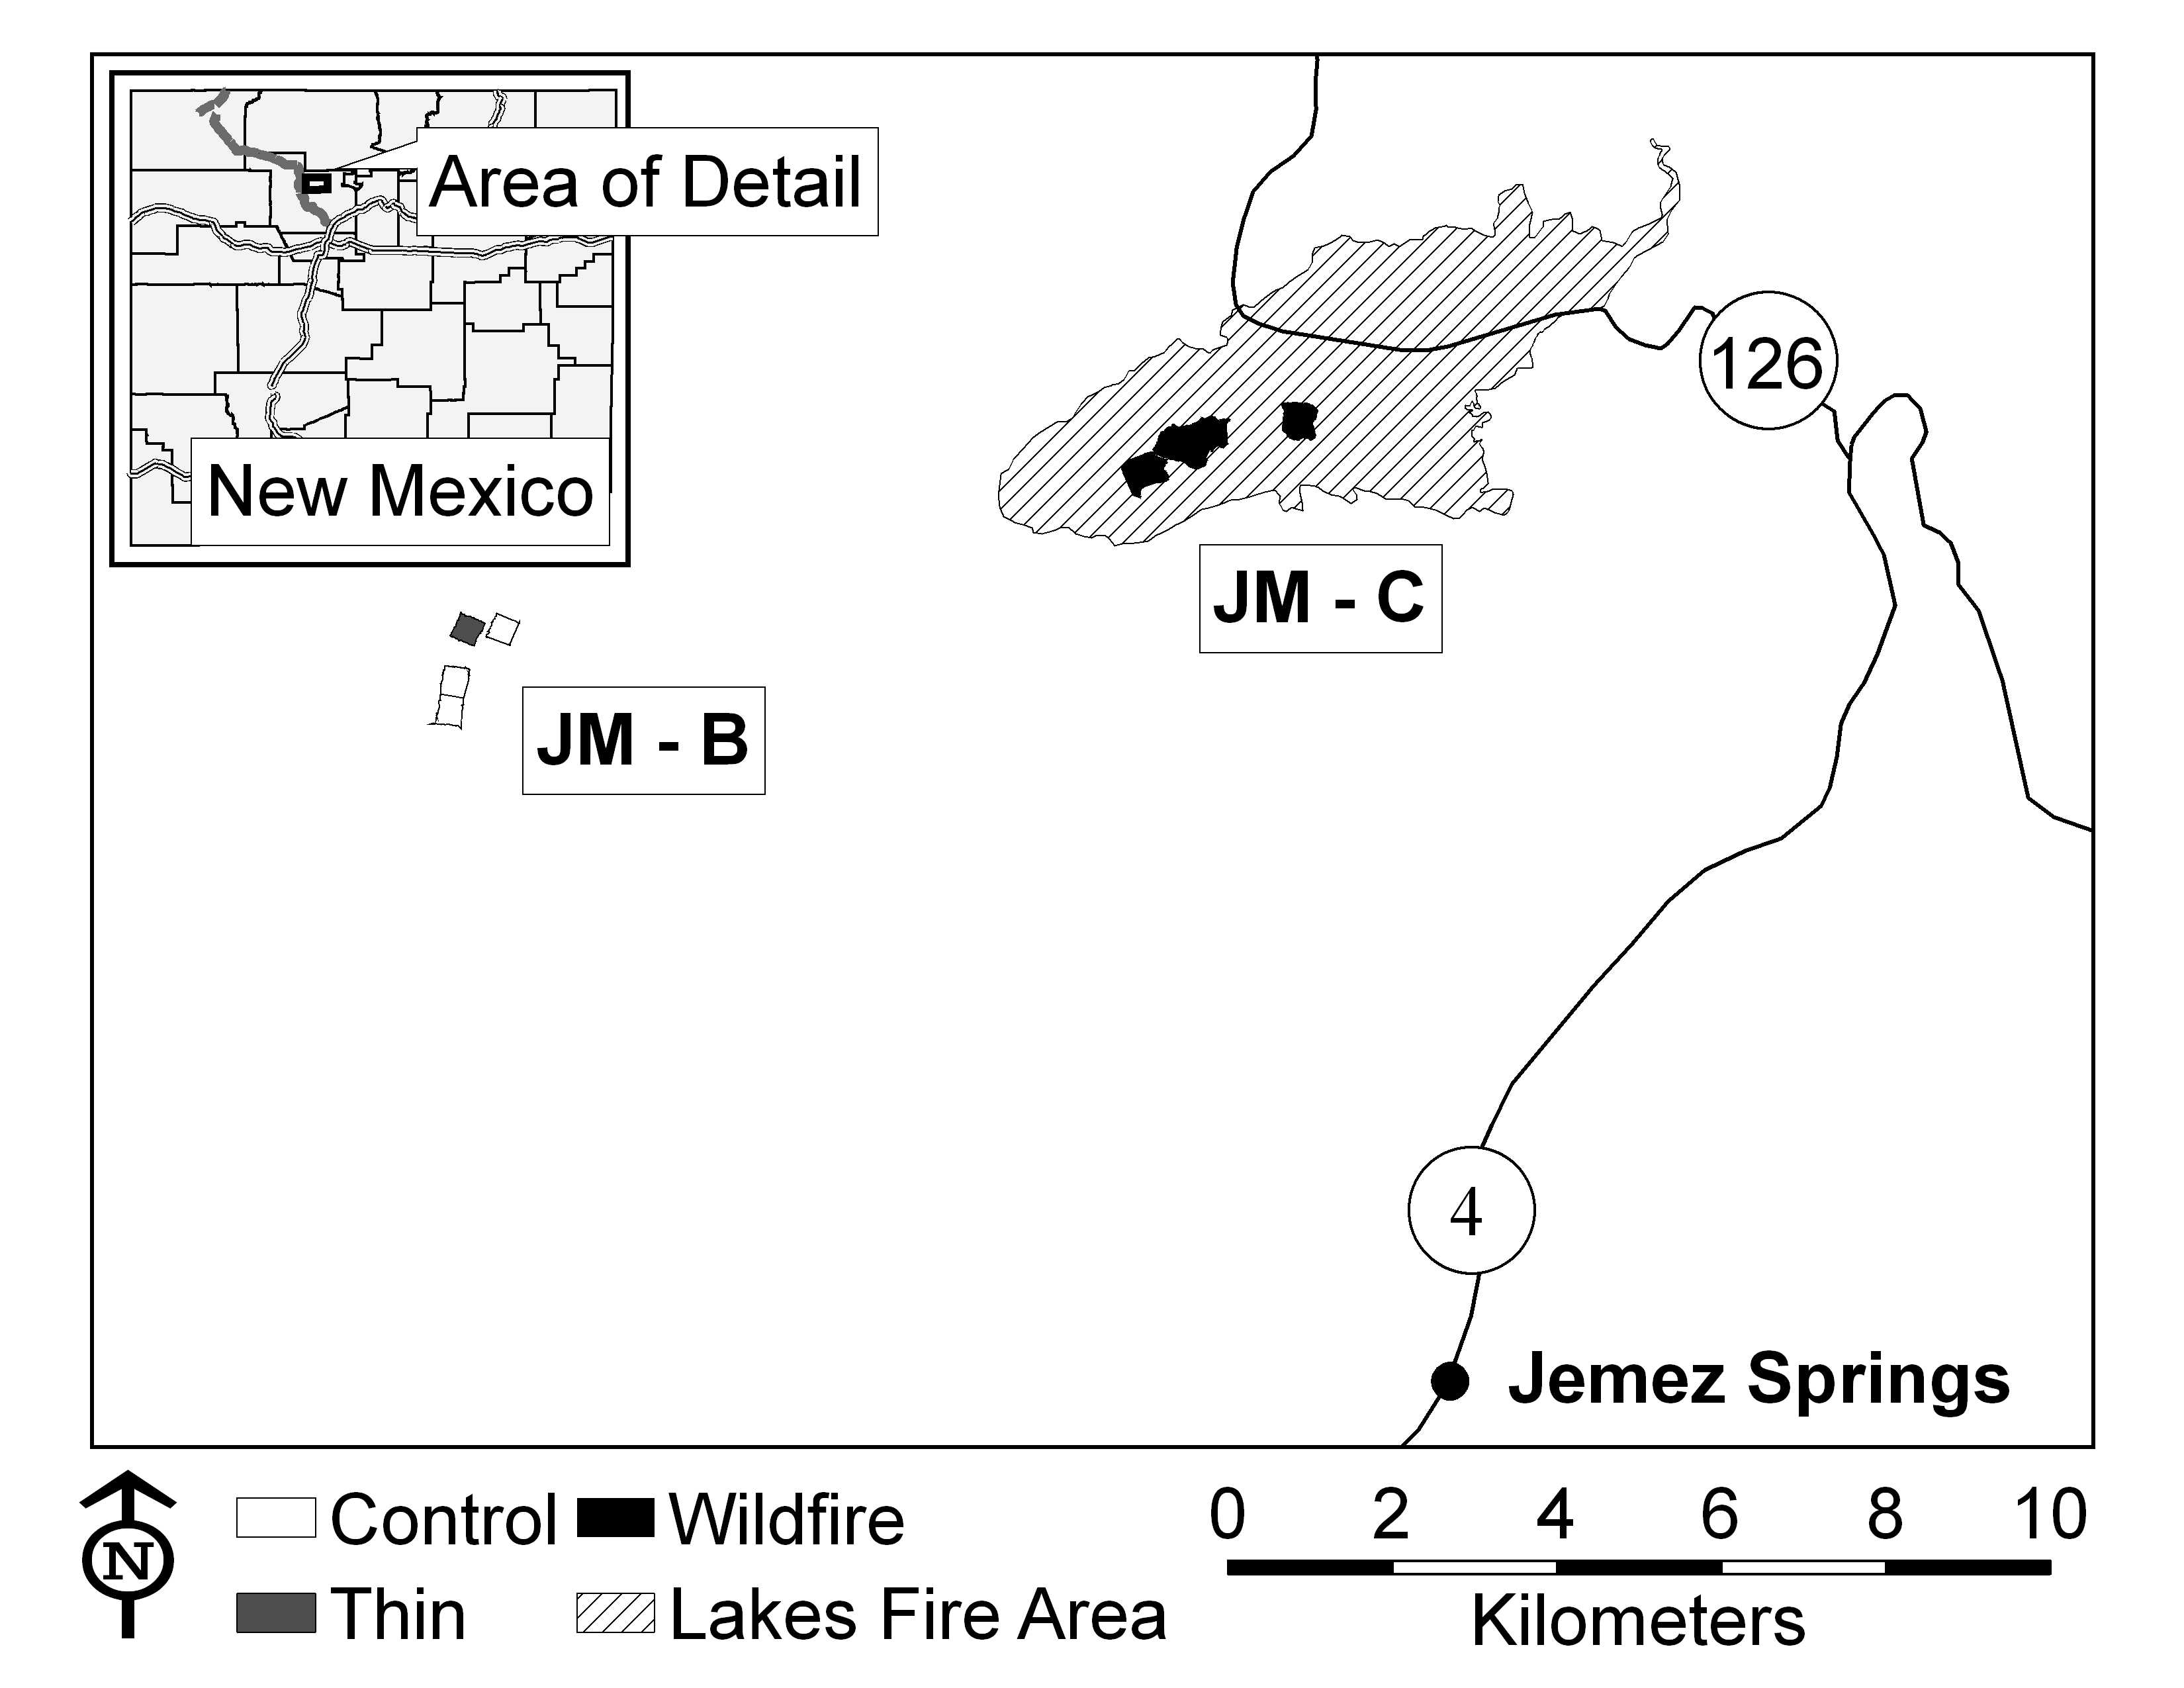
\includegraphics[height=4in,width=5.2in]{Ch14-Multisession/figs/converse_NM_Overview_4.jpg}
\end{center}
\caption{
Central New Mexico Study Area from \citet{converse_etal:2006jwm}.
}
\label{fig.studyarea}
\end{figure}



\begin{figure}[ht]
\begin{center}
\includegraphics[height=4.8in,width=6.5in]{Ch14-Multisession/figs/figure_V2.pdf}
\end{center}
\caption{
Abundance estimates for Peromyscus spp. per experimental unit
(with area = 5.0625 ha) for each of 24 groups composed of 8
experimental units in year 1 (groups 1:8), and the same 8
experimental units in year 2 (groups 9:16) and year 3 (groups 17:24)
(from \citet{royle_converse:2013}).
 Point estimates
(filled circles) are posterior modes, and error bars reflect 95\%
credible intervals. Also shown are the number of individuals
captured per group (open circles).  }
\label{fig.fig1}
\end{figure}

\end{comment}









